\documentclass[compress]{beamer}
\usepackage[utf8]{inputenc}
\usepackage[english]{babel}
\usepackage{hyperref}
\usepackage{ccicons}

\usepackage{tikz}
\usetikzlibrary{graphs, quotes, arrows.meta, matrix}

\newcommand\scalemath[2]{\scalebox{#1}{\mbox{\ensuremath{\displaystyle #2}}}}

\usetheme{default}
\usecolortheme{Nord}
\setbeamertemplate{navigation symbols}{}

\title{Teoria dei grafi}
\subtitle{Introduzione e primi algoritmi}
\author{Lorenzo Ferrari, Davide Bartoli}
\date{\today}

\begin{document}

\begin{frame}
  \maketitle
\end{frame}

\begin{frame}{Table of contents}
  \tableofcontents
\end{frame}


\section{Introduzione}

\subsection{Esempi}

\begin{frame}{Esempi}
  \begin{columns}
    \column{0.5\textwidth}
    \begin{center}
    \scalebox{0.7}{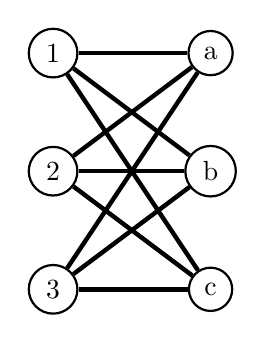
\begin{tikzpicture}
  \tikzset{vertex/.style = {draw, circle, thick}}
  \tikzset{arc/.style = {ultra thick}}
  % Nodes
  \node[vertex] (1) at (0, 3) {1};
  \node[vertex] (2) at (0, 1.5) {2};
  \node[vertex] (3) at (0, 0) {3};
  \node[vertex] (4) at (2, 3) {a};
  \node[vertex] (5) at (2, 1.5) {b};
  \node[vertex] (6) at (2, 0) {c};
  % Edges
  \draw[arc] (1) edge (4);
  \draw[arc] (1) edge (5);
  \draw[arc] (1) edge (6);
  \draw[arc] (2) edge (4);
  \draw[arc] (2) edge (5);
  \draw[arc] (2) edge (6);
  \draw[arc] (3) edge (4);
  \draw[arc] (3) edge (5);
  \draw[arc] (3) edge (6);
\end{tikzpicture}
}
    \end{center}
    \begin{center}
    \scalebox{0.7}{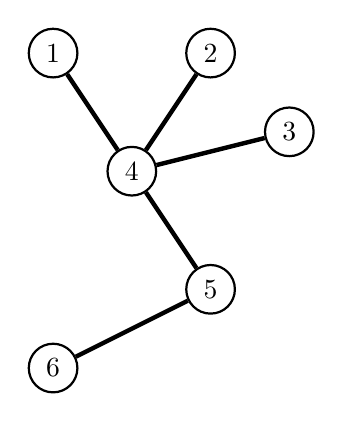
\begin{tikzpicture}
  \tikzset{vertex/.style = {draw, circle, thick}}
  \tikzset{arc/.style = {ultra thick}}
  % Nodes
  \node[vertex] (1) at (0, 4) {1};
  \node[vertex] (2) at (2, 4) {2};
  \node[vertex] (3) at (3, 3) {3};
  \node[vertex] (4) at (1, 2.5) {4};
  \node[vertex] (5) at (2, 1) {5};
  \node[vertex] (6) at (0, 0) {6};
  % Edges
  \draw[arc] (1) edge (4);
  \draw[arc] (2) edge (4);
  \draw[arc] (3) edge (4);
  \draw[arc] (4) edge (5);
  \draw[arc] (5) edge (6);
\end{tikzpicture}
}
    \end{center}
    \column{0.5\textwidth}
    \begin{center}
    \scalebox{0.7}{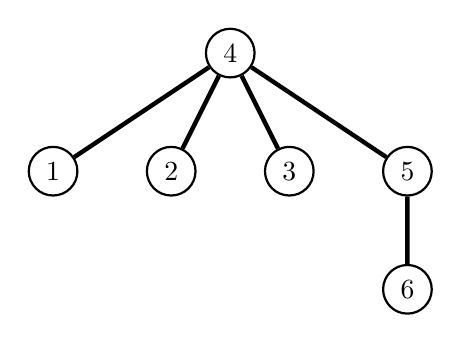
\begin{tikzpicture}
  \tikzset{vertex/.style = {draw, circle, thick}}
  \tikzset{arc/.style = {ultra thick}}
  % Actual tree
  \node[vertex] {4}
    child[arc] {node[vertex] {1}}
    child[arc] {node[vertex] {2}}
    child[arc] {node[vertex] {3}}
    child[arc] {node[vertex] {5}
      child[arc] {node[vertex] {6}}};
\end{tikzpicture}
}
    \end{center}
    \begin{center}
    \scalebox{0.7}{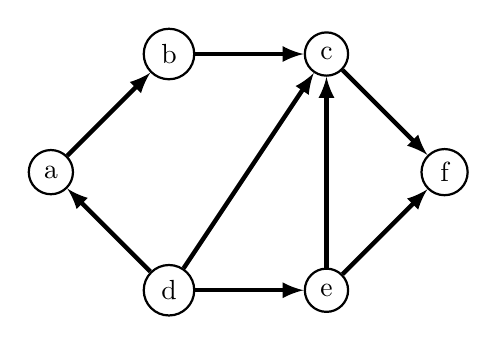
\begin{tikzpicture}
  \tikzset{vertex/.style = {draw, circle, thick}}
  \tikzset{arc/.style = {-latex, ultra thick}}
  % Nodes
  \node[vertex] (1) at (0, 1.5) {a};
  \node[vertex] (2) at (1.5, 3) {b};
  \node[vertex] (3) at (3.5, 3) {c};
  \node[vertex] (4) at (1.5, 0) {d};
  \node[vertex] (5) at (3.5, 0) {e};
  \node[vertex] (6) at (5, 1.5) {f};
  % Edges
  \draw[arc] (1) edge (2);
  \draw[arc] (2) edge (3);
  \draw[arc] (3) edge (6);
  \draw[arc] (4) edge (1);
  \draw[arc] (4) edge (3);
  \draw[arc] (4) edge (5);
  \draw[arc] (5) edge (3);
  \draw[arc] (5) edge (6);
\end{tikzpicture}
}
    \end{center}
  \end{columns}
\end{frame}

\begin{frame}[fragile]{Perch\`e studiamo i grafi?}
  \begin{alertblock}{}
    \begin{itemize}
    \item Tantissimi problemi possono essere ridotti a grafi
    \item I grafi sono bellissimi \verb|\(^-^)/|
    \end{itemize}
  \end{alertblock}
  \pause
  Tutto \`e grafo. I grafi trovano applicazione nelle aree pi\`u disparate.
\end{frame}

\begin{frame}{Esempi di problemi}
    \begin{itemize}
        \item Data la descrizione di una citt\`a, trova il cammino pi\`u breve da $A$ a $B$ (o determina che \`e impossibile raggiungere $B$ da $A$)
        \item Ci sono $N$ citt\`a e conosci la distanza tra ogni coppia di citt\`a. Per costruire una strada che collega due citt\`a il costo \`e direttamente proporzionale alla distanza. Trova il costo minimo per connettere tutte e $N$ le citt\`a.
        \item Date relazioni di dipendenza del tipo ``il pacchetto $x_i$ va installato prima del pacchetto $y_i$'', trova un ordine per installare tutti i pacchetti o determina che \`e impossibile.
    \end{itemize}
\end{frame}

\subsection{Definizioni}
\begin{frame}{Definizioni}{Grafo}
  \begin{block}{\textbf{Grafo} $G = (V, E)$}
    Un grafo \`e definito da due insiemi:
    \begin{itemize}
    \item $V$ \`e l'insieme dei \textbf{nodi}/\textbf{vertici}
    \item $E$ \`e l'insieme degli \textbf{archi}
  \end{itemize}
\end{block}
\end{frame}

\begin{frame}{Definizioni}{Nodi e Archi}
  \begin{block}{\textbf{Nodo}}
      \begin{itemize}
          \item Talvolta chiamati anche \emph{vertici}
          \item ogni nodo ha una label (un nome univoco)
    \end{itemize}
  \end{block}
  \pause
  \begin{block}{\textbf{Arco}}
      \begin{itemize}
        \item Ogni arco \`e definito da una coppia di nodi
        \item Un arco connette i nodi che lo definiscono
        \item In alcuni casi, un arco pu\`e connettere un nodo a se stesso
        \item In alcuni casi, un arco pu\`o avere un peso
  \end{itemize}
\end{block}
\end{frame}

\begin{frame}{}
    \begin{exampleblock}{Esempio}
    \begin{itemize}
    \item $G = (V, E)$
    \item $V = \{1, 2, 3, 4\}$
    \item $E = \{(1,2), (1,3), (1,4), (2,4), (3,4)\}$
    \end{itemize}
  \end{exampleblock}
  \begin{center}
  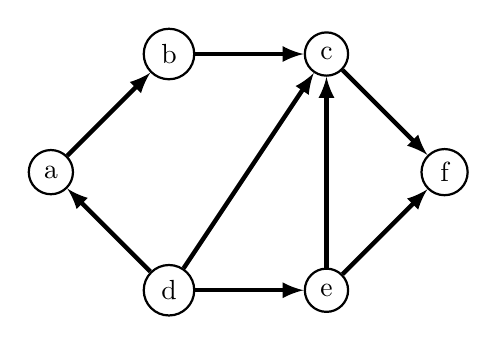
\begin{tikzpicture}
  \tikzset{vertex/.style = {draw, circle, thick}}
  \tikzset{arc/.style = {-latex, ultra thick}}
  % Nodes
  \node[vertex] (1) at (0, 1.5) {a};
  \node[vertex] (2) at (1.5, 3) {b};
  \node[vertex] (3) at (3.5, 3) {c};
  \node[vertex] (4) at (1.5, 0) {d};
  \node[vertex] (5) at (3.5, 0) {e};
  \node[vertex] (6) at (5, 1.5) {f};
  % Edges
  \draw[arc] (1) edge (2);
  \draw[arc] (2) edge (3);
  \draw[arc] (3) edge (6);
  \draw[arc] (4) edge (1);
  \draw[arc] (4) edge (3);
  \draw[arc] (4) edge (5);
  \draw[arc] (5) edge (3);
  \draw[arc] (5) edge (6);
\end{tikzpicture}

  \end{center}
\end{frame}

\begin{frame}{Definizioni}{Cammini e Cicli}
  \begin{block}{\textbf{Cammino}}
    Un cammino di lunghezza $n$ in un grafo $G = (V, E)$ \`e una sequenza di nodi $v_0, \dots, v_n \in V$ tale che 
    \[
        (v_{i-1}, v_i) \in E \ \forall \ 1 \leq i \leq n.
    \]

    Un cammino si dice \emph{semplice} se tutti i $v_i$ sono diversi uno dall'altro.
  \end{block}
  \pause
  \begin{block}{\textbf{Ciclo}}
    Un ciclo \`e un cammino in cui il primo e l'ultimo nodo coincidono.
  \end{block}
\end{frame}

\begin{frame}{Definizioni}{Sottografo}
  \begin{block}{\textbf{Sottografo}}
    Un grafo $G' = (V', E')$ \`e sottografo di $G = (V, E)$ se e soltanto se $V' \subseteq V$ e $E' \subseteq E$.
  \end{block}
  \begin{columns}
  \column{0.5\textwidth}
  \begin{center}
  \scalebox{0.7}{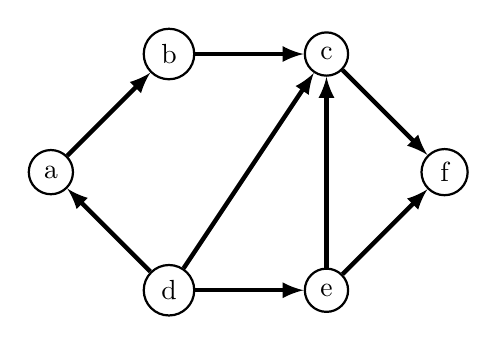
\begin{tikzpicture}
  \tikzset{vertex/.style = {draw, circle, thick}}
  \tikzset{arc/.style = {-latex, ultra thick}}
  % Nodes
  \node[vertex] (1) at (0, 1.5) {a};
  \node[vertex] (2) at (1.5, 3) {b};
  \node[vertex] (3) at (3.5, 3) {c};
  \node[vertex] (4) at (1.5, 0) {d};
  \node[vertex] (5) at (3.5, 0) {e};
  \node[vertex] (6) at (5, 1.5) {f};
  % Edges
  \draw[arc] (1) edge (2);
  \draw[arc] (2) edge (3);
  \draw[arc] (3) edge (6);
  \draw[arc] (4) edge (1);
  \draw[arc] (4) edge (3);
  \draw[arc] (4) edge (5);
  \draw[arc] (5) edge (3);
  \draw[arc] (5) edge (6);
\end{tikzpicture}
}
  \end{center}
  \column{0.5\textwidth}
  \begin{center}
  \scalebox{0.7}{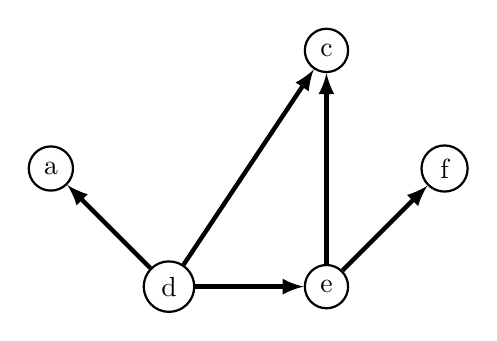
\begin{tikzpicture}
  \tikzset{vertex/.style = {draw, circle, thick}}
  \tikzset{arc/.style = {-latex, ultra thick}}
  % Nodes
  \node[vertex] (1) at (0, 1.5) {a};
  % \node[vertex] (2) at (1.5, 3) {b};
  \node[vertex] (3) at (3.5, 3) {c};
  \node[vertex] (4) at (1.5, 0) {d};
  \node[vertex] (5) at (3.5, 0) {e};
  \node[vertex] (6) at (5, 1.5) {f};
  % Edges
  % \draw[arc] (1) edge (2);
  % \draw[arc] (2) edge (3);
  % \draw[arc] (3) edge (6);
  \draw[arc] (4) edge (1);
  \draw[arc] (4) edge (3);
  \draw[arc] (4) edge (5);
  \draw[arc] (5) edge (3);
  \draw[arc] (5) edge (6);
\end{tikzpicture}
}
  \end{center}
  \end{columns}
\end{frame}

\begin{frame}{Dimensioni di un grafo}
  \begin{block}{\textbf{Definizioni}}
    \begin{itemize}
      \item $n = |V|$: numero di nodi
      \item $m = |E|$: numero di archi
    \end{itemize}
  \end{block}
  \pause
    \begin{block}{\textbf{Relaioni tra $n$ e $m$}}
        \begin{itemize}
          \item In un grafo non diretto, $m \leq \frac{n(n-1)}{2} = O(n^2)$
          \item In un grafo diretto, $m \leq n^2 - n = O(n^2)$
        \end{itemize}
    \end{block}
\end{frame}

\subsection{Tipologie di grafi}
\begin{frame}[fragile]{Grafi diretti e non diretti}
  \begin{columns}
  \column{0.5\textwidth}
  \begin{block}{\textbf{Grafi diretti} $G = (V, E)$}
    \begin{itemize}
      \item $E$ \`e un insieme di coppie \emph{ordinate} di nodi $(u, v)$
    \end{itemize}
  \end{block}
  \begin{verbatim}
V = { a,b,c,d,e,f }
E = { (a,b),(a,d),(b,c),
      (d,a),(d,c),(d,e),
      (e,c) }
  \end{verbatim}
  \begin{center}
  \scalebox{0.65}{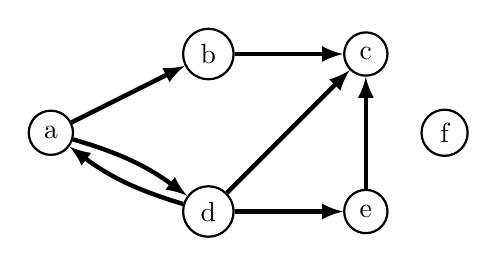
\begin{tikzpicture}
  \tikzset{vertex/.style = {draw, circle, thick}}
  \tikzset{arc/.style = {-latex, ultra thick}}
  % Nodes
  \node[vertex] (1) at (0, 1) {a};
  \node[vertex] (2) at (2, 2) {b};
  \node[vertex] (3) at (4, 2) {c};
  \node[vertex] (4) at (2, 0) {d};
  \node[vertex] (5) at (4, 0) {e};
  \node[vertex] (6) at (5, 1) {f};
  % Edges
  \draw[arc] (1) edge (2);
  \draw[arc] (2) edge (3);
  \draw[arc] (4) edge (3);
  \draw[arc] (4) edge (5);
  \draw[arc] (5) edge (3);
  \draw[arc, bend left = 10] (1) edge (4);
  \draw[arc, bend left = 10] (4) edge (1);
\end{tikzpicture}
}
  \end{center}
  \column{0.5\textwidth}
  \begin{block}{\textbf{Grafi indiretti} $G = (V, E)$}
    \begin{itemize}
      \item $E$ \`e un insieme di coppie \emph{non ordinate} di nodi $[u, v]$
    \end{itemize}
  \end{block}
  \begin{verbatim}
V = { a,b,c,d,e,f }
E = { [a,b],[a,d],[b,c],
      [c,d],[c,e],[e,d] }

  \end{verbatim}
  \begin{center}
  \scalebox{0.65}{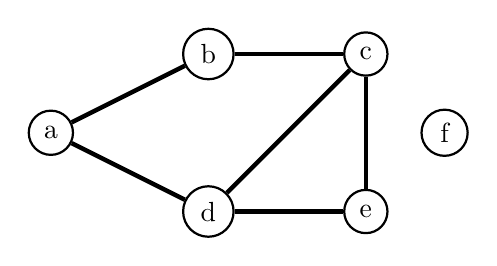
\begin{tikzpicture}
  \tikzset{vertex/.style = {draw, circle, thick}}
  \tikzset{arc/.style = {ultra thick}}
  % Nodes
  \node[vertex] (1) at (0, 1) {a};
  \node[vertex] (2) at (2, 2) {b};
  \node[vertex] (3) at (4, 2) {c};
  \node[vertex] (4) at (2, 0) {d};
  \node[vertex] (5) at (4, 0) {e};
  \node[vertex] (6) at (5, 1) {f};
  % Edges
  \draw[arc] (1) edge (2);
  \draw[arc] (2) edge (3);
  \draw[arc] (4) edge (3);
  \draw[arc] (4) edge (5);
  \draw[arc] (5) edge (3);
  \draw[arc] (1) edge (4);
\end{tikzpicture}
}
  \end{center}
\end{columns}
\end{frame}

\begin{frame}{Grafi ciclici e aciclici}
  \begin{columns}
    \column{0.5\textwidth}
    \begin{block}{\textbf{Grafo ciclico}}
      \begin{itemize}
        \item Contiene dei cicli
      \end{itemize}
    \end{block}
    \begin{center}
    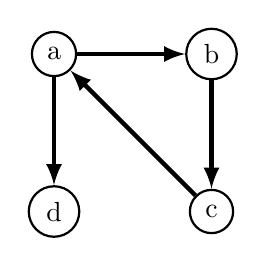
\begin{tikzpicture}
  \tikzset{vertex/.style = {draw, circle, thick}}
  \tikzset{arc/.style = {-latex, ultra thick}}
  % Nodes
  \node[vertex] (1) at (0, 2) {a};
  \node[vertex] (2) at (2, 2) {b};
  \node[vertex] (3) at (2, 0) {c};
  \node[vertex] (4) at (0, 0) {d};
  % Edges
  \draw[arc] (1) edge (2);
  \draw[arc] (1) edge (4);
  \draw[arc] (2) edge (3);
  \draw[arc] (3) edge (1);
\end{tikzpicture}

  \end{center}
    \column{0.5\textwidth}
    \begin{block}{\textbf{Grafo aciclico}}
      \begin{itemize}
        \item Non contiene cicli
      \end{itemize}
    \end{block}
    \begin{center}
    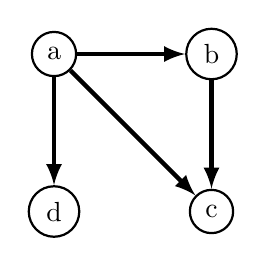
\begin{tikzpicture}
  \tikzset{vertex/.style = {draw, circle, thick}}
  \tikzset{arc/.style = {-latex, ultra thick}}
  % Nodes
  \node[vertex] (1) at (0, 2) {a};
  \node[vertex] (2) at (2, 2) {b};
  \node[vertex] (3) at (2, 0) {c};
  \node[vertex] (4) at (0, 0) {d};
  % Edges
  \draw[arc] (1) edge (2);
  \draw[arc] (1) edge (4);
  \draw[arc] (1) edge (3);
  \draw[arc] (2) edge (3);
\end{tikzpicture}

    \end{center}
  \end{columns}
\end{frame}

\begin{frame}{Grafi ciclici e aciclici}
  \begin{columns}
    \column{0.5\textwidth}
    \begin{block}{\textbf{Grafo ciclico}}
      \begin{itemize}
        \item Contiene dei cicli
      \end{itemize}
    \end{block}
    \begin{center}
    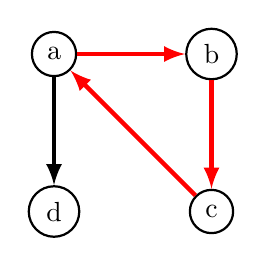
\begin{tikzpicture}
  \tikzset{vertex/.style = {draw, circle, thick}}
  \tikzset{arc/.style = {-latex, ultra thick}}
  % Nodes
  \node[vertex] (1) at (0, 2) {a};
  \node[vertex] (2) at (2, 2) {b};
  \node[vertex] (3) at (2, 0) {c};
  \node[vertex] (4) at (0, 0) {d};
  % Edges
  \draw[arc] (1) edge[red] (2);
  \draw[arc] (1) edge (4);
  \draw[arc] (2) edge[red] (3);
  \draw[arc] (3) edge[red] (1);
\end{tikzpicture}

  \end{center}
    \column{0.5\textwidth}
    \begin{block}{\textbf{Grafo aciclico}}
      \begin{itemize}
        \item Non contiene cicli
      \end{itemize}
    \end{block}
    \begin{center}
    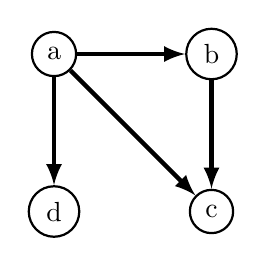
\begin{tikzpicture}
  \tikzset{vertex/.style = {draw, circle, thick}}
  \tikzset{arc/.style = {-latex, ultra thick}}
  % Nodes
  \node[vertex] (1) at (0, 2) {a};
  \node[vertex] (2) at (2, 2) {b};
  \node[vertex] (3) at (2, 0) {c};
  \node[vertex] (4) at (0, 0) {d};
  % Edges
  \draw[arc] (1) edge (2);
  \draw[arc] (1) edge (4);
  \draw[arc] (1) edge (3);
  \draw[arc] (2) edge (3);
\end{tikzpicture}

    \end{center}
  \end{columns}
\end{frame}

\begin{frame}{Grafi pesati}
  \begin{block}{\textbf{Grafo pesato}}
    \begin{itemize}
      \item a ogni arco \`e associato un \emph{peso}
      \item generalmente il peso indica il costo di percorrere quell'arco
    \end{itemize}
  \end{block}
  \begin{center}
  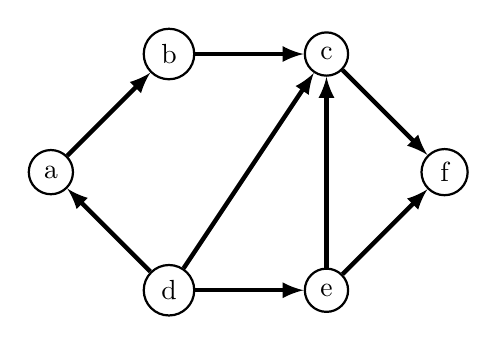
\begin{tikzpicture}
  \tikzset{vertex/.style = {draw, circle, thick}}
  \tikzset{arc/.style = {-latex, ultra thick}}
  % Nodes
  \node[vertex] (1) at (0, 1.5) {a};
  \node[vertex] (2) at (1.5, 3) {b};
  \node[vertex] (3) at (3.5, 3) {c};
  \node[vertex] (4) at (1.5, 0) {d};
  \node[vertex] (5) at (3.5, 0) {e};
  \node[vertex] (6) at (5, 1.5) {f};
  % Edges
  \draw[arc] (1) edge (2);
  \draw[arc] (2) edge (3);
  \draw[arc] (3) edge (6);
  \draw[arc] (4) edge (1);
  \draw[arc] (4) edge (3);
  \draw[arc] (4) edge (5);
  \draw[arc] (5) edge (3);
  \draw[arc] (5) edge (6);
\end{tikzpicture}

  \end{center}
\end{frame}

\begin{frame}{Alberi}
  \begin{columns}
    \column{0.5\textwidth}
    \begin{block}{\textbf{Albero}}
      \begin{itemize}
      \item Grafo \emph{connesso} con $m = n - 1$
      \end{itemize}
    \end{block}
    \begin{center}
    \scalebox{0.7}{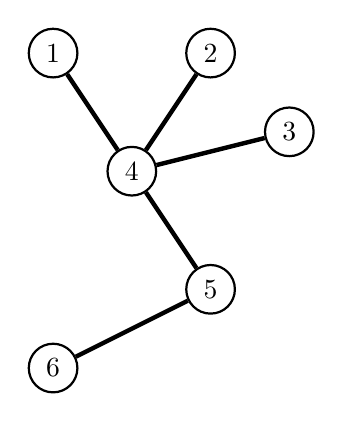
\begin{tikzpicture}
  \tikzset{vertex/.style = {draw, circle, thick}}
  \tikzset{arc/.style = {ultra thick}}
  % Nodes
  \node[vertex] (1) at (0, 4) {1};
  \node[vertex] (2) at (2, 4) {2};
  \node[vertex] (3) at (3, 3) {3};
  \node[vertex] (4) at (1, 2.5) {4};
  \node[vertex] (5) at (2, 1) {5};
  \node[vertex] (6) at (0, 0) {6};
  % Edges
  \draw[arc] (1) edge (4);
  \draw[arc] (2) edge (4);
  \draw[arc] (3) edge (4);
  \draw[arc] (4) edge (5);
  \draw[arc] (5) edge (6);
\end{tikzpicture}
}
    \end{center}
    \column{0.5\textwidth}
    \begin{block}{\textbf{Albero radicato}}
      \begin{itemize}
          \item Grafo \emph{connesso} con $m = n - 1$ e in cui un nodo \`e la \textbf{radice}
      \end{itemize}
    \end{block}
    \begin{center}
    \scalebox{0.8}{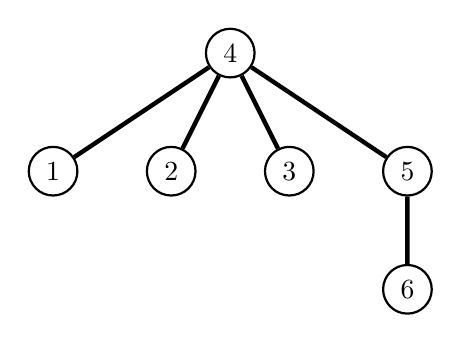
\begin{tikzpicture}
  \tikzset{vertex/.style = {draw, circle, thick}}
  \tikzset{arc/.style = {ultra thick}}
  % Actual tree
  \node[vertex] {4}
    child[arc] {node[vertex] {1}}
    child[arc] {node[vertex] {2}}
    child[arc] {node[vertex] {3}}
    child[arc] {node[vertex] {5}
      child[arc] {node[vertex] {6}}};
\end{tikzpicture}
}
    \end{center}
  \end{columns}
  Caratteristica: un albero non presenta cicli.
\end{frame}

\subsection{Rappresentazione di grafi}

\begin{frame}{Rappresentazioni}
  \begin{block}{}
    Ci sono due implementazioni ``classiche''.
  \end{block}
  \begin{itemize}
      \pause
    \item Matrici di adiacenza
    \item Liste di adiacenza
  \end{itemize}
\end{frame}

\begin{frame}{Matrice di adiacenza}
  \begin{columns}
    \column{0.5\textwidth}
    \[
    m_{uv} = \begin{cases}
      1, & \text{se $(u,v) \in E$} \\
      0, & \text{se $(u,v) \notin E$}
    \end{cases}
    \]
    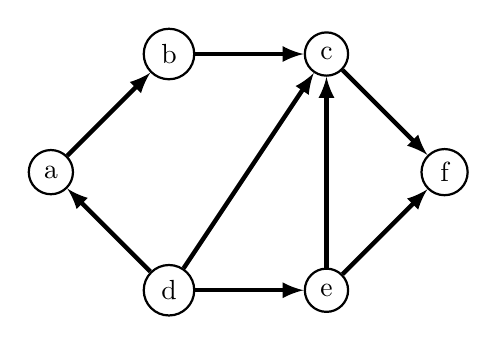
\begin{tikzpicture}
  \tikzset{vertex/.style = {draw, circle, thick}}
  \tikzset{arc/.style = {-latex, ultra thick}}
  % Nodes
  \node[vertex] (1) at (0, 1.5) {a};
  \node[vertex] (2) at (1.5, 3) {b};
  \node[vertex] (3) at (3.5, 3) {c};
  \node[vertex] (4) at (1.5, 0) {d};
  \node[vertex] (5) at (3.5, 0) {e};
  \node[vertex] (6) at (5, 1.5) {f};
  % Edges
  \draw[arc] (1) edge (2);
  \draw[arc] (2) edge (3);
  \draw[arc] (3) edge (6);
  \draw[arc] (4) edge (1);
  \draw[arc] (4) edge (3);
  \draw[arc] (4) edge (5);
  \draw[arc] (5) edge (3);
  \draw[arc] (5) edge (6);
\end{tikzpicture}

    \column{0.5\textwidth}
    \[
    \begin{matrix}
       & \textbf{0} & \textbf{1} & \textbf{2} & \textbf{3} & \textbf{4} \\
      \textbf{0} & 0 & 1 & 0 & 0 & 0 \\
      \textbf{1} & 0 & 0 & 1 & 0 & 0 \\
      \textbf{2} & 0 & 0 & 0 & 0 & 1 \\
      \textbf{3} & 1 & 0 & 1 & 0 & 1 \\
      \textbf{4} & 0 & 0 & 1 & 0 & 0
    \end{matrix}
    \]
  \end{columns}
\end{frame}

\begin{frame}{Lista di adiacenza}
  \begin{columns}
  \column{0.5\textwidth}
  \[G.adj(u) = \{v \ : \ (u,v) \in E\}\]
  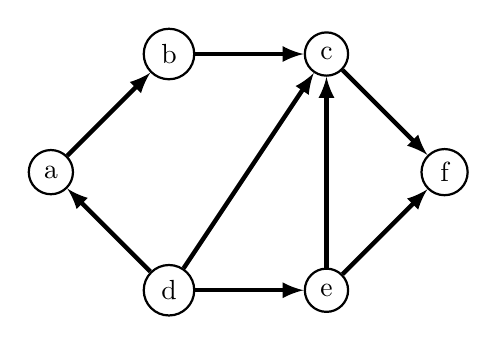
\begin{tikzpicture}
  \tikzset{vertex/.style = {draw, circle, thick}}
  \tikzset{arc/.style = {-latex, ultra thick}}
  % Nodes
  \node[vertex] (1) at (0, 1.5) {a};
  \node[vertex] (2) at (1.5, 3) {b};
  \node[vertex] (3) at (3.5, 3) {c};
  \node[vertex] (4) at (1.5, 0) {d};
  \node[vertex] (5) at (3.5, 0) {e};
  \node[vertex] (6) at (5, 1.5) {f};
  % Edges
  \draw[arc] (1) edge (2);
  \draw[arc] (2) edge (3);
  \draw[arc] (3) edge (6);
  \draw[arc] (4) edge (1);
  \draw[arc] (4) edge (3);
  \draw[arc] (4) edge (5);
  \draw[arc] (5) edge (3);
  \draw[arc] (5) edge (6);
\end{tikzpicture}

  \column{0.5\textwidth}
  $\scalemath{1.8}{\fbox{0} \rightarrow \fbox{1}}$ \\
  $\scalemath{1.8}{\fbox{1} \rightarrow \fbox{2}}$ \\
  $\scalemath{1.8}{\fbox{2} \rightarrow \fbox{4}}$ \\
  $\scalemath{1.8}{\fbox{3} \rightarrow \fbox{0}\fbox{2}\fbox{4}}$ \\
  $\scalemath{1.8}{\fbox{4} \rightarrow \fbox{2}}$
  \end{columns}
\end{frame}

\section{Visite su un grafo}

\subsection{BFS}
\begin{frame}{Breadth-first search}
  \begin{block}{\textbf{Problema}}
    Dato un grafo $G = (V, E)$ e un vertice $r \in V$ (radice), visitare esattamente una
     volta tutti i vertici del grafo che si possono raggiungere da $r$.
  \end{block}
  \begin{block}{\textbf{Breadth-first search (BFS)}}
    Attraversa il grafo visitando i nodi per livelli: prima i nodi a distanza 1 dalla radice, poi a distanza 2, etc.\\
    Alcune applicazioni:

    \begin{itemize}
    \item percorso minimo tra due nodi
    \item componenti connesse
    \end{itemize}
  \end{block}
\end{frame}

\begin{frame}[fragile]{Breadth-first search}
    \makebox[\textwidth]{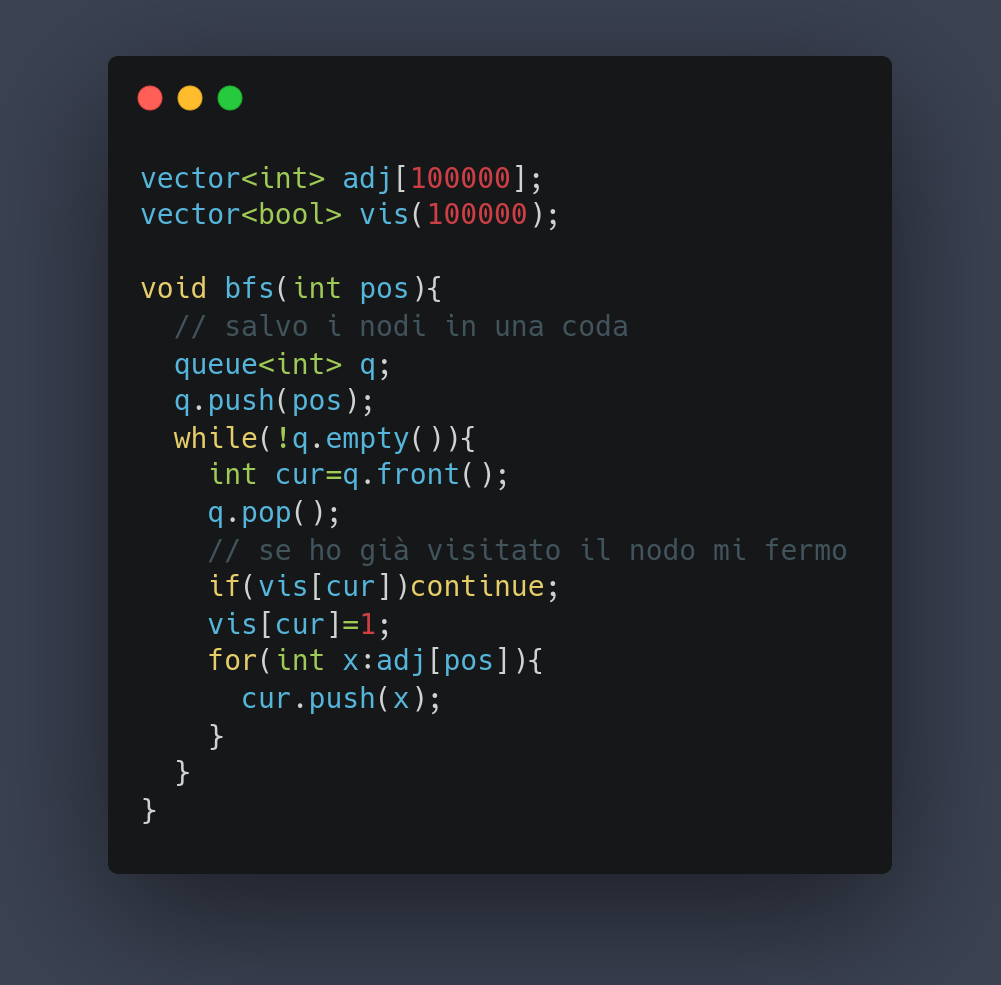
\includegraphics[scale=.28]{./img/bfs.png}}
\end{frame}

\subsection{DFS}
\begin{frame}{Depth-first search}
  \begin{block}{\textbf{Problema}}
    Dato un grafo $G = (V, E)$ e un vertice $r \in V$ (radice), visitare esattamente una
     volta tutti i vertici del grafo che si possono raggiungere da $r$.
  \end{block}
  \begin{block}{\textbf{Depth-first search (DFS)}}
    Attraversa il grafo visitando tutti i nodi raggiungibili da un nodo, poi tutti i noti raggiungibili da quei nodi...
    Applicazioni:
    \begin{itemize}
    \item topological sort
    \item trovare cicli
    \item componenti connesse
    \item componenti fortemente connesse
    \end{itemize}
  \end{block}
\end{frame}

\begin{frame}[fragile]{Depth-first search}
    \makebox[\textwidth]{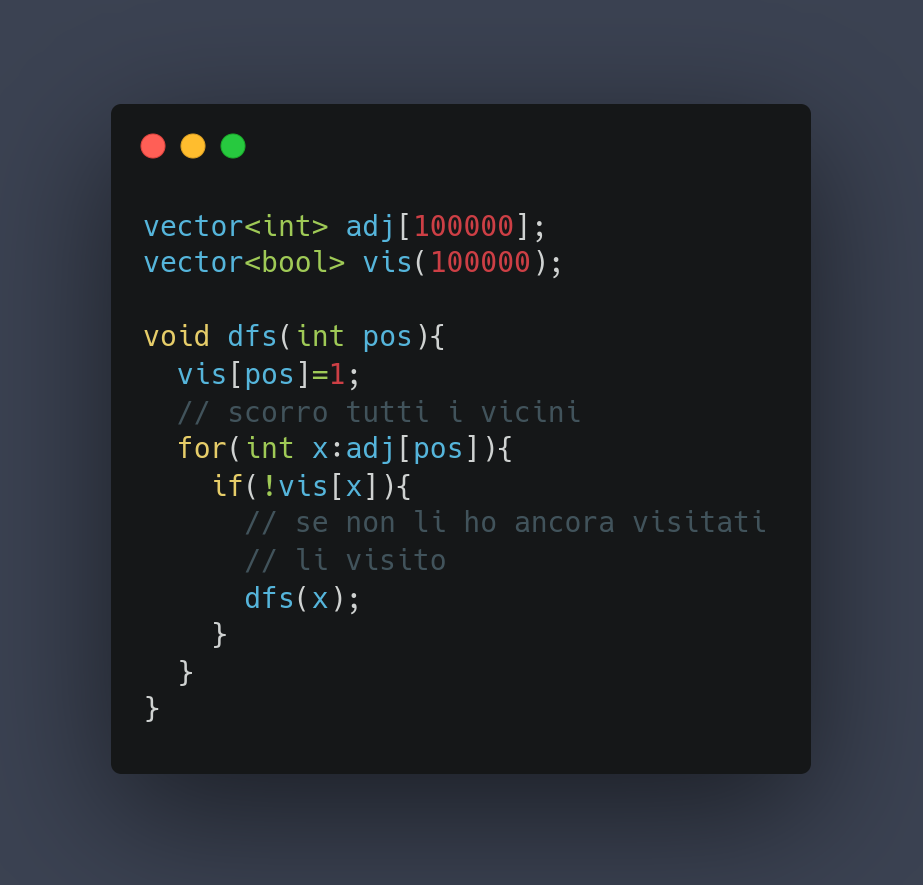
\includegraphics[scale=.30]{./img/dfs.png}}
\end{frame}

\section{Problemi}

\subsection{Componenti connesse}
\begin{frame}{Componenti connesse}
  \begin{block}{\textbf{Problema}}
    Dato un grafo $G = (V, E)$ non diretto, trovare il numero di componenti connesse.
  \end{block}
  \begin{center}
  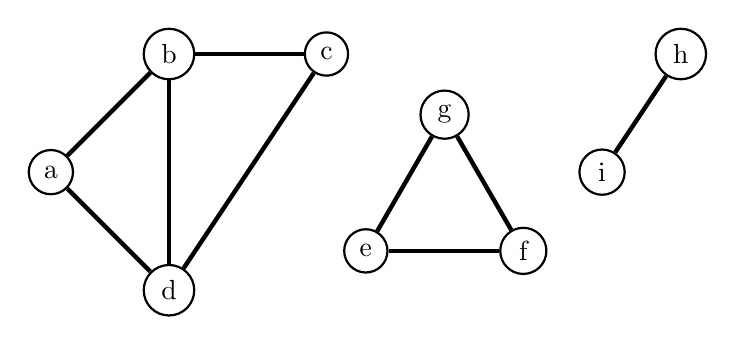
\begin{tikzpicture}
  \tikzset{vertex/.style = {draw, circle, thick}}
  \tikzset{arc/.style = {ultra thick}}
  % Component 1
  \node[vertex] (1) at (0, 1.5) {a};
  \node[vertex] (2) at (1.5, 3) {b};
  \node[vertex] (3) at (3.5, 3) {c};
  \node[vertex] (4) at (1.5, 0) {d};
  \draw[arc] (1) edge (2);
  \draw[arc] (1) edge (4);
  \draw[arc] (2) edge (3);
  \draw[arc] (2) edge (4);
  \draw[arc] (3) edge (4);
  % work in progress
  % \draw[blue, dashed, rounded corners = 8pt] (1) -- (2) -- (3) -- (4) -- (1);
  % Component 2
  \node[vertex] (5) at (4, 0.5) {e};
  \node[vertex] (6) at (6, 0.5) {f};
  \node[vertex] (7) at (5, 2.23) {g};
  \draw[arc] (5) edge (6);
  \draw[arc] (5) edge (7);
  \draw[arc] (6) edge (7);
  % Component 3
  \node[vertex] (8) at (8, 3) {h};
  \node[vertex] (9) at (7, 1.5) {i};
  \draw[arc] (8) edge (9);
\end{tikzpicture}

  \end{center}
\end{frame}

\begin{frame}{Componenti connesse}
    Come possiamo contare il numero di componenti connesse?
    \pause
    Possiamo utilizzare una delle 2 visite viste prima (BFS e DFS).
    \pause
    \begin{itemize}
        \item iteriamo su tutti i nodi, se non sono stati visitati, eseguiamo una visita
        \pause
        \item in questo modo visitiamo tutti i nodi della stessa componente connessa
        \pause
        \item il numero di visite effettuate \`e il numero di componenti connesse
    \end{itemize}
  \end{frame}

\begin{frame}{Problemi}{Ponti}
    \begin{exampleblock}{Ponti}
        Dato un grafo di $N \leq 10 \ 000$ e $M \leq 20 \ 000$ archi, trova il minimo numero di archi da costruire per rendere il grafo connesso.
    \end{exampleblock}
    \small{\underline{\url{https://training.olinfo.it/\#/task/ponti/statement}}}
    \pause
    \begin{itemize}
        \item se $M = 0$ la risposta \`e $N-1$
        \pause
        \item possiamo considerare ogni componente connessa come un nodo
        \pause
        \item se ci sono $K$ componenti connesse, la risposta \`e $K-1$
    \end{itemize}
\end{frame}

\begin{frame}{Problemi}{Ponti}
    \makebox[\textwidth]{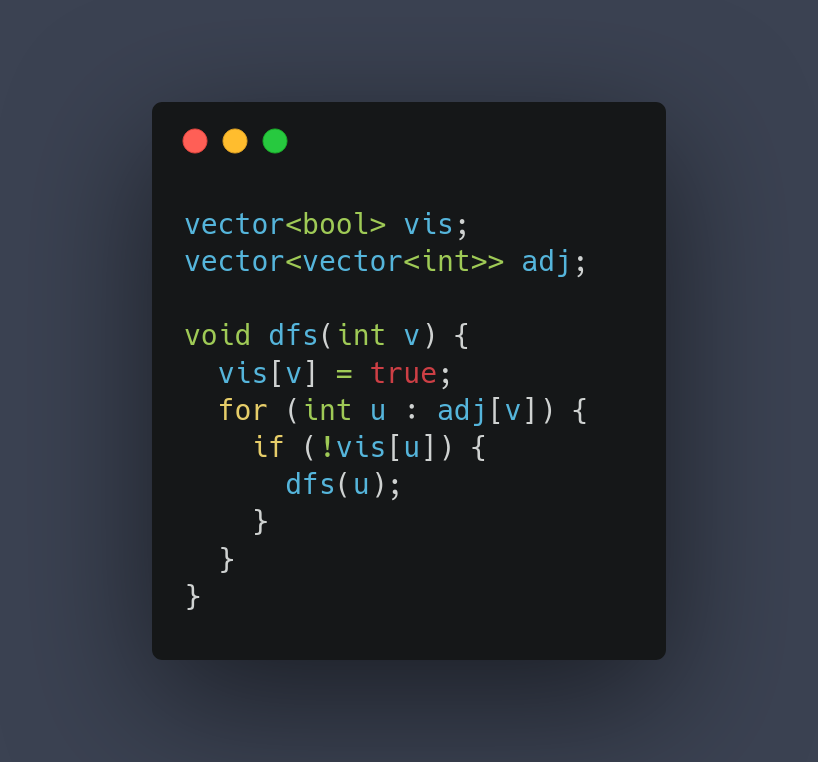
\includegraphics[scale=.3]{./img/dfs_ponti.png}}
\end{frame}

\begin{frame}
    \makebox[\textwidth]{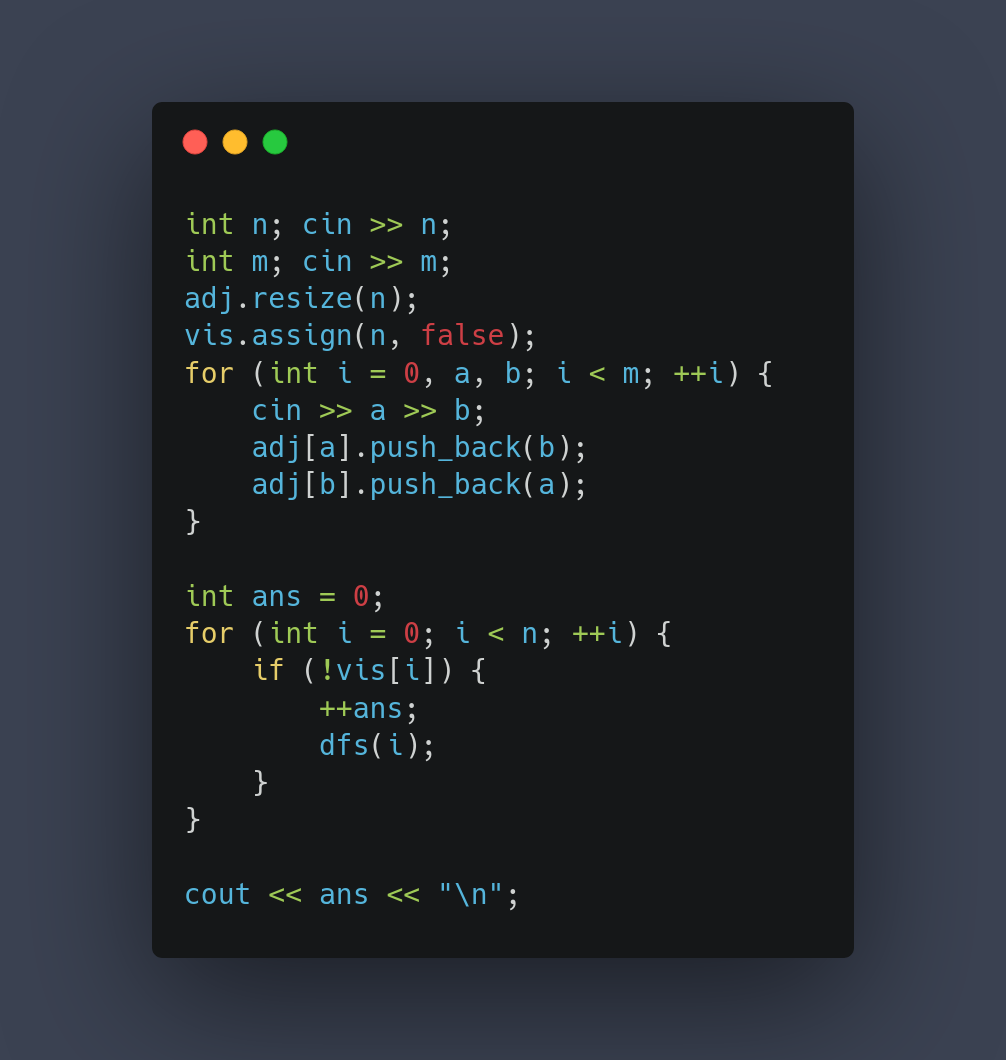
\includegraphics[scale=.25]{./img/main_ponti.png}}
\end{frame}

\begin{frame}{Distanza minima}
    \begin{exampleblock}{Problema}
        Dato un grafo $G = (V, E)$ non diretto, trovare la minima distanza tra due nodi $a$ e $b$, ovvero il minimo numero di 
        archi da attraversare per raggiungere $b$ partendo da $a$.
    \end{exampleblock}
    \pause
    \begin{itemize}
        \item Possiamo utilizzare una BFS, dato che visita i nodi ordinati per distanza dal nodo di partenza.
        \pause
        \item Nella coda della BFS teniamo il nodo attuale e la sua distanza da $a$.
        \pause
        \item Quando troviamo $b$, abbiamo trovato la distanza minima.
    \end{itemize}
\end{frame}

\begin{frame}{Domande?}
  \tableofcontents
\end{frame}

\begin{frame}{Problemi}{}
    \underline{\url{https://cses.fi/problemset/}}
    \underline{\url{https://training.olinfo.it/\#/task/ponti/statement}}
    \underline{\url{https://training.olinfo.it/\#/task/tecla/statement}}
    \underline{\url{https://training.olinfo.it/\#/task/sentieri/statement}}
\end{frame}

\end{document}
